\documentclass{book}
\usepackage[a4paper,top=2.0cm,bottom=2.0cm,left=2.0cm,right=3.0cm]{geometry}

%\documentclass[pdftex,10pt,a4paper]{book}
%\usepackage[paperwidth=19cm,
%paperheight=26cm, outer=2cm, 
%top=1.5cm, bottom=1.5cm]{ geometry}

\usepackage[english,italian]{babel} %l'ultima lingua è quella che legge per i titoli
\usepackage[utf8]{inputenc}
\usepackage[T1]{fontenc,url}
\usepackage{titlesec}
\usepackage{easylist}
\usepackage{hanging}

\usepackage[pdftex,colorlinks]{hyperref}
\hypersetup{
	colorlinks=true,
	linkcolor=black,
	filecolor=magenta,
	urlcolor=cyan,
}
\usepackage{hypcap}
\usepackage{blindtext}
\usepackage{tipa}
\usepackage{epigraph}
\usepackage{enumerate}
\usepackage{longtable}
\usepackage{setspace}
\usepackage{verbatim}
\usepackage{graphicx}
\usepackage{amsmath}
\usepackage{pbox}
\usepackage{fancyhdr}
\usepackage{cancel}
\usepackage{tabularx}
\usepackage{booktabs}
\usepackage{multirow}
\usepackage{longtable}
\usepackage{tikz}
\usepackage{tikz-qtree}
\usepackage{subfig}
\usepackage{xcolor}
\usepackage{amssymb}
\usepackage{amsmath}
\usepackage{mathrsfs}
\usepackage{textcomp}
\usepackage{circuitikz}
\usepackage{pifont}
\usepackage{imakeidx}
\usepackage{verbatim}
\usepackage{dsfont}
\usepackage{listings}
\usepackage{color}
\usepackage{upgreek}
\usepackage{tasks}
\usepackage{exsheets}
\usepackage{pgfplots}
\usepackage{amsthm}
\usepackage{wasysym}
\usepackage{chemfig}

\usepackage{showframe}
\renewcommand\ShowFrameLinethickness{0.15pt}
%\renewcommand*\ShowFrameColor{\color{red}}

%\usepackage{showkeys} %serve per mostrare le etichette "tag" o target, va tolta per la versione definitiva;

\newtheorem{definizione}{Definizione}
\newtheorem{Teoria}{Teoria}
\SetupExSheets[question]{type=exam}

\definecolor{mygreen}{rgb}{0,0.6,0}
\definecolor{mygray}{rgb}{0.5,0.5,0.5}
\definecolor{mymauve}{rgb}{0.58,0,0.82}

\lstset{ 
  backgroundcolor=\color{white},   % choose the background color; you must add \usepackage{color} or \usepackage{xcolor}; should come as last argument
  basicstyle=\footnotesize,        % the size of the fonts that are used for the code
  breakatwhitespace=false,         % sets if automatic breaks should only happen at whitespace
  breaklines=true,                 % sets automatic line breaking
  captionpos=b,                    % sets the caption-position to bottom
  commentstyle=\color{mygreen},    % comment style
  deletekeywords={...},            % if you want to delete keywords from the given language
  escapeinside={\%*}{*)},          % if you want to add LaTeX within your code
  extendedchars=true,              % lets you use non-ASCII characters; for 8-bits encodings only, does not work with UTF-8
  firstnumber=1000,                % start line enumeration with line 1000
  frame=single,	                   % adds a frame around the code
  keepspaces=true,                 % keeps spaces in text, useful for keeping indentation of code (possibly needs columns=flexible)
  keywordstyle=\color{blue},       % keyword style
  language=Octave,                 % the language of the code
  morekeywords={*,...},            % if you want to add more keywords to the set
  numbers=left,                    % where to put the line-numbers; possible values are (none, left, right)
  numbersep=5pt,                   % how far the line-numbers are from the code
  numberstyle=\tiny\color{mygray}, % the style that is used for the line-numbers
  rulecolor=\color{black},         % if not set, the frame-color may be changed on line-breaks within not-black text (e.g. comments (green here))
  showspaces=false,                % show spaces everywhere adding particular underscores; it overrides 'showstringspaces'
  showstringspaces=false,          % underline spaces within strings only
  showtabs=false,                  % show tabs within strings adding particular underscores
  stepnumber=2,                    % the step between two line-numbers. If it's 1, each line will be numbered
  stringstyle=\color{mymauve},     % string literal style
  tabsize=2,	                   % sets default tabsize to 2 spaces
  title=\lstname                   % show the filename of files included with \lstinputlisting; also try caption instead of title
}

\linespread{1.2} % l'interlinea

\frenchspacing

\newcommand{\abs}[1]{\lvert#1\rvert}

\usepackage{floatflt,epsfig}

\usepackage{multicol}
\newcommand\yellowbigsqcup[1][\displaystyle]{%
  \fboxrule0pt
  \ifx#1\textstyle\fboxsep-0.6pt\else\fboxsep-1.25pt\fi
  \mathrel{\fcolorbox{white}{yellow}{$#1\bigsqcup$}}}

\title{Appunti di Chimica:\\ Per ingegneria}
\author{Nicola Ferru}
\date{}
\makeindex[columns=3, title=Alphabetical Index, intoc]

\begin{document}
\maketitle
\tableofcontents
\listoftables
\listoffigures
\chapter{Introduzione}
La chimica è la scienza che studia la composizione, la struttura e le trasformazioni della \textit{MATERIA}\\
La Materia
\begin{enumerate}
	\item Composizione (analisi qualitativa e qualitativa)
	\item Struttura-proprietà (es. diamante-grafite)
	\item Modellizzazione e progettazione
\end{enumerate}
Le trasformazione della Materia
\begin{enumerate}
	\item Corrosione (\textbf{es. ferro-ruggine})
	\item Combustione (es. sorgenti di energia)
	\item Sintesi (es. farmaci, pigmenti, nanomateriali, polimeri\dots)
\end{enumerate}
\begin{figure}[h]
	\centering
	\Tree[.Universo [.Energia ciò\ che\ occupa\ spazio\ e\ ha\ massa  ] [.Materia Capacità\ di\ \underline{eseguire un lavoro} ] ]
	\caption{suddivisione tra energia e materia}
	\label{fig:enmat1}
\end{figure}
Un sistema è una porzione delimitata di spazio che rappresenta l’oggetto dello studio mentre l’ambiente è tutto ciò che sta attorno al sistema: l’insieme di sistema e ambiente costituisce l’Universo.
\section{Gli stati della materia}
La materia possiede sostanzialmente tre stati:
\begin{enumerate}
	\item \textit{Solida} - ha una forma definita e un volume proprio;
	\item \textit{Liquido} - ha un volume ma non possiede una forma propria;
	\item \textit{Gas} - non ha né forma, né un volume proprio, si espande in modo da riempire il contenitore che lo contiene.
\end{enumerate}
\section{Proprietà fisiche}
\begin{definizione} 
	Proprietà che possono essere osservate e misurate SENZA alterare la composizione della sostanza
\end{definizione}
\begin{enumerate}
	\item colore;
	\item punto di fusione e di ebollizione;
	\item indice di rifrazione;
	\item densità.
\end{enumerate}
\section{Trasformazioni della materia}
\subsection{Trasformazioni Fisiche}
\begin{definizione}
	Trasformazioni che avvengono senza alterare la composizione della sostanza
\end{definizione}
Esempi di trasformazione fisiche:
\begin{tasks}{2}
	\task ebollizione di un liquido;
	\task fusione di un solido;
	\task sciogliere un solido in un liquido per ottenere una miscela omogenea (ovvero una \textbf{soluzione})
\end{tasks}
\subsection{Trasformazioni Chimiche}
\begin{definizione}
	Trasformazioni che avvengono \texttt{alterando} la natura delle sostanze coinvolte e portando alla formazione di nuovi composti.
\end{definizione}
Un esempio di questo tipo di trasformazione: La combustione del metano. Si parte dal metano e dal ossigeno e si arriva a biossido di carbonio e acqua:
\begin{equation*}
	CH_4+ 2O_2\to CO_2+2H_2O
\end{equation*}
Al termine della trasformazione abbiamo una sostanza differente da quella di partenza, in alcuni casi la procedura non è reversibile.
\section{Sostanza pure}
\begin{definizione}
	Una mataria che ha una composizione omogenea non può essere scomposto tramite una trasformazione fisica in materiali differenti. In quanto non è possibile scomporre ulteriormente la materia
\end{definizione}
\begin{figure}[h]
	\centering
	\Tree [.Può\ essere\ scomposta\ Chimicamente\ in\ sostanze\ più\ semplici? [.Composto ] [.Elemento ] ]
	\caption{Sostanza pura suddivisione}
	\label{fig:Sostanza pura suddivisione}
\end{figure}
\begin{enumerate}
	\item Composto - sostanza formato da almeno due tipi di atomi;
	\item Elemento - tutti gli atomi la costituiscono sono dello stesso tipo.
\end{enumerate}
\begin{table}[htp]
\begin{center}
\begin{tabular}{|c|c|}
	\hline
	Composti&Elemento\\\hline\hline
	Acqua $H_2O$&Ossigeno $O_2$\\
	Anidride carbonica $CO_2$&Diamante $C$\\
	Cloruro di sodio $NaCl$&\\
	Benzene $C_6H_6$&\\
	Etanolo $C_2H_5OH$&\\\hline
\end{tabular}
\end{center}
\caption{Sostanza pura suddivisione}
\label{tab:Sostanza pura suddivisione}
\end{table}%
\section{Miscela}
Composti di Due o più sostanze pure
\chapter{Stechiometria}
\begin{definizione}
La stechiometria è la branca della chimica che studia i rapporti quantitativi (rapporti ponderali) delle sostanze chimiche nelle reazioni chimiche.\\
By \href{https://it.wikipedia.org/wiki/Stechiometria}{Wikipedia}
\end{definizione}
Da questa definizione è chiaro che questo sistema verrà utilizzato per una
serie di esercizi potenzialmente presenti all'esame.\\
Calcolo delle quantità di sostanza consumata o prodotte durante una reazione chimica. Le equazioni chimiche danno una rappresentazione \underline{qualitativa} (ci dicono quali sostanza prendono parte) e \underline{quantitativa} (in quali rapporti ponderali) dei processi chimici.
\begin{equation}
	\text{\color{blue}Reagente } \boxed{\color{blue}NH_3}\to\boxed{{\color{orange}N_2}+{\color{orange}H_2}} \text{ \color{orange}Prodotti}
\end{equation}
Per avere una rappresentazione quantitativa è fondamentale \underline{BILANCIARE} correttamente l'equazione usando gli opportuni \textit{coefficienti stechiometrici}.
\begin{equation}
	{\color{red}2}NH_3\to{\color{orange}N_2}+{\color{red}3}{\color{orange}H_2} \text{ \textit{coefficienti stechiometrici}} 
\end{equation}
\textit{I coefficienti stechiometrici} sono numeri interi che indicano quante moli (o molare, atomi o ioni) reagiscono (se si tratta di un prodotto) durante la reazione chimica.
\section{Bilanciamento di un'equazione chimica}
Le trasformazioni chimiche rispettano le \textit{{\color{blue}legge della conservazione della massa} o {\color{blue}legge di Lavoisier}.} Per bilanciare un'equazione chimica si deve avere che:
\begin{itemize}
\item per ciascun elemento, gli atomi presenti tra i reagenti devono essere in numero \textbf{UGUALE} a quelli presenti tra i prodotti;
\item se la reazione coinvolge specie ioniche, somma delle cariche elettriche dei reagenti, deve essere uguale a quella dei prodotti.
\end{itemize}
\begin{center}
	METODO PER TENTATIVI SUCCESSIVI
\end{center}
Si basa su una attenta osservazione dell'equazione non bilanciata:
\begin{equation}
	Ca(OH)_2+H_3PO_4\to Ca_3(PO_4)_2+H_2O
\end{equation}
Si attribuiscono i coefficienti stechiometrici facendo in modo che il numero e il tipo degli atomi presenti tra i reagenti, siano uguali a quelli presenti a destra della freccia:
\begin{equation}
	3Ca(OH)_2+2H_3PO_4\to Ca_3(PO_4)_2+6H_2O
\end{equation}
\section{Resa o rendimento di una reazione}
Non sempre le reazioni precedono fino a \textbf{completamento}, cioè fino a quando i reagenti (almeno quello limitante) sono completamente convertiti nei prodotti. Inoltre, si possono avere delle reazioni secondarie che portano i reagenti a trasformarsi in prodotti diversi da quelli riportati nell'equazione.\\
\textbf{\color{red}In questi casi le quantità di prodotti ottenute, risultano inferiori alla quantità teoriche (stechiometriche).}\\
Si definisce \textbf{resa} o \textbf{rendimento percentuale} (r) di una reazione chimica il rapporto (moltiplicato per cento) il rapporto tra la quantità di prodotto effettivamente ottenere ($Q_e$) e quella che si sarebbe avuta se la reazione fosse andata a completamente (resa teorica $Q_t$):
\begin{equation}
	r=\frac{Q_e}{Q_t}*100
\end{equation}

\chapter{Modelli atomici}
\section{Teoria atomica di Dalton}
\begin{itemize}
\item La materia è composta da particelle piccolissime e indivisibili: gli Atomi
\item Tutti gli atomi di uno stesso elemento hanno la \underline{stessa} messa e le \underline{stesse} proprietà (sono identici)
\item Atomi di elementi diversi hanno masse differenti
\item Gli atomi sono indistruttibili e mantengono la loro identità le reazioni chimiche
\item Gli atomi si combinano tra loro secondo rapporti definiti e costanti, espressi da numeri interi
\end{itemize}
\section{Modello atomico di Thomson}
\subsection{Basi sperimentali:}
\begin{itemize}
\item Studi sull'effetto del passaggio dell'elettricità sui gas
\item Elettrolisi
\item Scoperta della radioattività
\end{itemize}
Forniscono evidenza che particelle cariche sono costituenti fondamentali della materia.
\subsection{Esperimento di Thomson}
Misura del rapporto carica/massa dell'elettrone
\begin{equation}
	\frac{e}{m}=1.7588*10^{11}C/Kg
\end{equation}
\subsubsection{Esperimento di Millikan}
Misura degli cariche dell'elettrone
\begin{equation}
	e=1.602*10^{-19}C
\end{equation}
\subsection{Modello atomitco di Thomson}
\begin{Teoria}
	Atomi costituiti da una nuvola di carica positiva neutralizzata da elettroni in un modello a panettone
\end{Teoria}
Il modello <<Plum pudding>>      
\section{Esperimento di Rutherford}
Esperimento di Rutherford sulla sulla deviazione di particelle $\alpha$ ($He^{2+}$) da parte di sottili lamine d'oro (600nm). Lampi di luce segnalano dove le particelle alfa hanno colipito lo schermo
\begin{figure}[!h]
  	\centering
	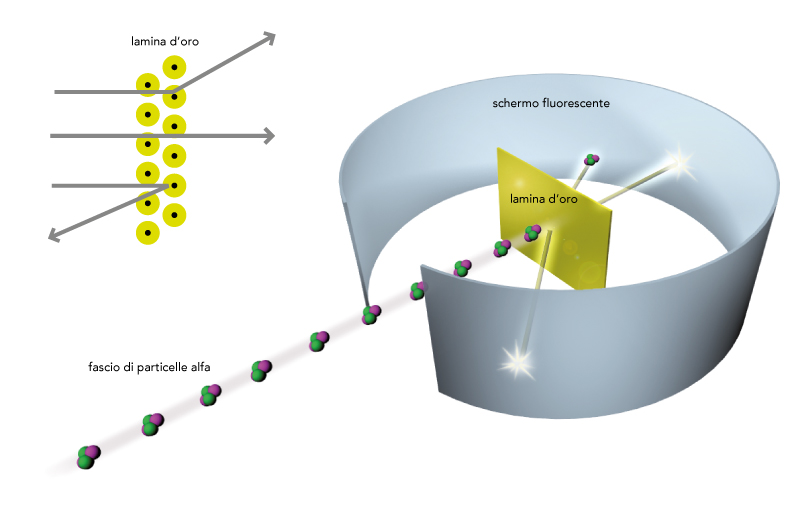
\includegraphics[height=6cm]{img/Esperimento di Rutherfor.jpg}
\end{figure}
Quindi da questo esperimento si che le ipotesi di Thomson erano errate, e quindi la nuova teoria è
\begin{Teoria}
	Atomo nucleare costituito da un nucleo formato da protoni e neutroni circondato da un numero di elettroni pari ai protoni.
\end{Teoria}
\subsection {punti critici}
Se gli elettroni sono stazionari l'attrazione elettrostatica dovrebbe partarli sul nucleo, se si muovono in un'orbita attorno portarli sul nucleo si instaura un dipolo oscillante che dissipa energia sotto forma di onda elettromagnetica con conseguente caduta dell'elettrone sul nucleo!
\subsubsection{<<Death-spiral of the electron>>}
Una particella in movimento ed elettricamente carica perde incessantemente energia, questo vale anche per l'elettrone ({\color{red} -}), perdendo via via energia avvrebbero finito per muoversi lungo orbite più piccole fino a cadere sul nucleo (\textbf{collassare}).
\subsection{Onda}
Un'onda è una perturbazione che nasce da una sorgente e si propaga \underline{TEMPO} e nello \underline{SPAZIO}, trasportando \underline{ENERGIA}
\begin{figure}[!h]
  	\centering
	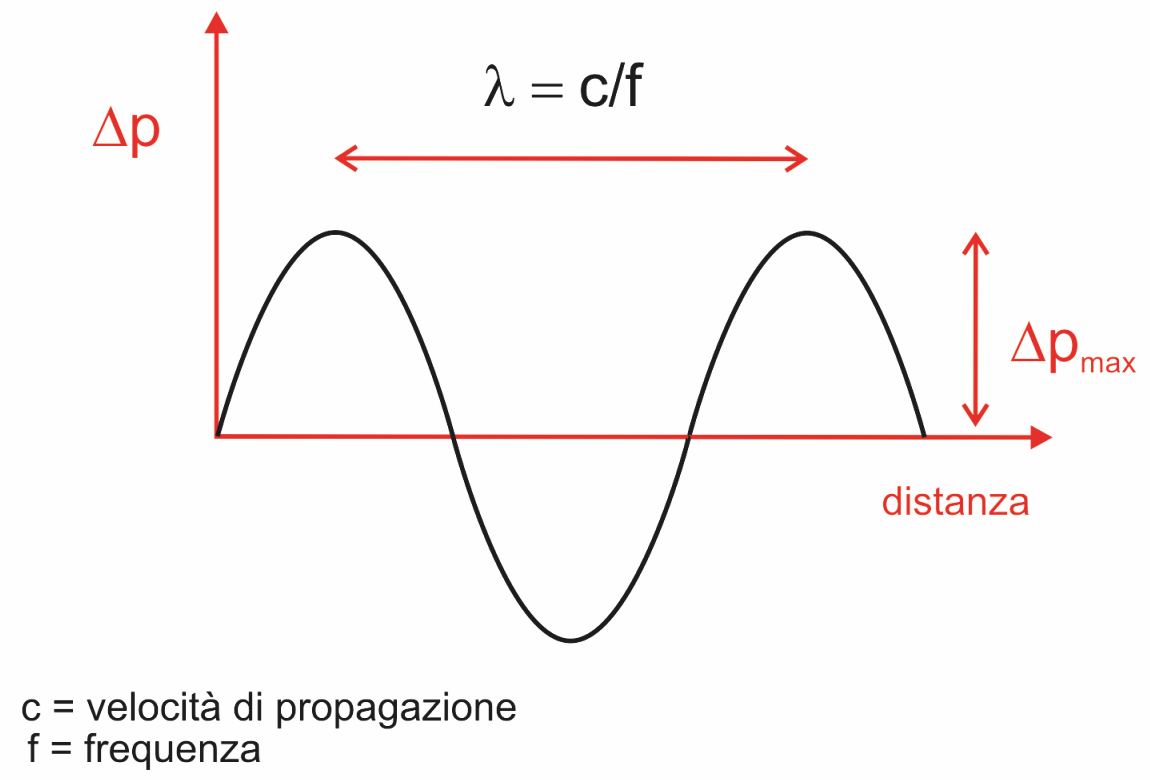
\includegraphics[height=6cm]{img/onda.png}
\end{figure}
$\lambda$ è la distanza tra due massimi o due minimi successivi.
\subsection{Onde Elettromagnetiche}
Una radiazione elettromagnetica può essere considerata come un campo elettromagnetico oscillazione che si propaga nello spazio.\\
\texttt{\color{red} La luce è una radiazione elettromagnetica, e ha quindi una natura ondulatoria.}\\
La luce consiste in un campo elettrico e un campo magnetico oscillanti e orientati perpendicolarmente tra loro e perpendicolarmente alla direzione di propagazione del raggio.
\subsubsection{Velocità di una radiazione elettromagnetica}
Nel vuoto una radiazione elettromagnetica si propaga alla velocità della luce
\begin{equation}
	\boxed{{\color{red}\lambda}*{\color{orange}v}=c} \text{ costante=}3.00x10^8m/sec (nel vuoto)
\end{equation}
\begin{itemize}
\item {\color{red}$\lambda$= lu}
\end{itemize}

\chapter{Proprietà periodiche}

\chapter{Soluzioni}

\chapter{Legame chimico}
\section{Introduzione}
In natura le soluzioni costituite da atomi isolati sono rare, di solito, gli
atomi si trovano combinati fra loro per formare dei \underline{Composti}.
Questi possono essere di tre tipi; 
\begin{itemize}
	\item \textit{Molecolare} - si basa sulla condivisione degli elettroni di
		valenza (quelli più esterni) da parte degli che danno origine al
		legamene. La forza che tiene uniti degli atomi deriva dall'attrazione
		che entrambi i nuclei esercitano sugli elettroni condivisi.\\
		\textbf{Esempio:} $H_2,\text{ }O_2 \text{ e } N_2$ dove gli atomi
		mettono in condivisione, rispettivamente, 1, 2 e 3 elettroni di valenza
		ciascuno.
	\item \textit{Ionico} - è dovuto alle forze di attrazione elettrostatica
		che si esercitano tra ioni di carica opposta.\\
		\textbf{Esempio:} $NaCl$ che è formato da cationi $Na^+$ e di anioni
		$Cl^-$.
	\item \textit{Metallico} - gli atomi sono tenuti uniti dagli elettroni di
		valenza che sono liberi di muoversi tra i cationi.\\
		\textbf{Esempio:} Sodio (Na), Oro (Au), Titanio (Ti), \dots
\end{itemize}
\subsection{Teorema di Lewis}
La reattività degli elementi è correlata alla tendenza di raggiungere la
configurazione elettronica del gas nobile più vicino ({\color{red} otteziale} o
doppietto per He). Questa tendenza è nota come \underline{Regola dell'Ottetto}.
\begin{enumerate}
	\item Gli \textbf{elettroni di valenza} giocano un ruolo fondamentale nel
		formare legame chimico;
	\item La condivisione di una o più coppie di elettroni porta alla
		formazione di legami covalenti;
	\item Il trasferimento elettronico da un atomo {\color{red}A} ad uno
		{\color{blue}B} porta al legame ionico.
\end{enumerate}
\begin{equation}
	2Na_{(s)}+Cl_{2(g)}\to 2Na^++2Cl
\end{equation}
Rappresenta il simbolo di elemento circondato da un numero di punti pari al
numero degli elettroni di valenza.
\subsection{Struttura di Lewis}
\begin{table}[h!]
  \centering
	\begin{tabular}{lcl}
		&Elettroni del core&Elettroni di valenza\\\hline
		Boro&\charge{0=\.,90=\.,180=\.}{B}&$1s^22s^22p^1$\\
		&&Core = [He]\\
		&&valenza = $2s^2\text{ }2p^1$\\
		Bromine&\charge{0=\:,90=\:,180=\.,270=\:}{B}&$1s^22s^2\text{
		}2p^63s^2\text{ }3d^{10}4s^24p^5$\\
		&&core = $[Ar]3d^{10}$\\
		&&valenza = $4s^24p^5$
		\\\hline
	\end{tabular}
	\caption{Comparazione tra elettroni core\\ ed elettroni di valenza}
\end{table}
\charge{0=\.,90=\.,180=\.}{B} $\to$ Simbolo di Lewis
\subsection{Elettronegatività \textit{x}}
Misura empirica della tendenza di un atomo in una molecola ad attrarre gli
elettroni di legame. Secondo \textit{Mulliken} è media dell'\textbf{affinità
elettronica} (tendenza ad attrarre un $e^-$ addizionale) e del
\textbf{potenziale di ionizzazione} (tendenza a mantenere l'$e^-$)
\begin{equation}
	x=\frac{(-\textbf{AE}+\textbf{EI})}{2}
\end{equation}
\textit{Si può prevedere se un legame chimico è ionico o covalente sulla base
della differenza di elettronegatività.}
\subsection{Elettronegatività di Pauling}
In una molecola \textbf{AB} la differenza di elettronegatività tra due atomi
\textbf{A} e \textbf{B} viene determinata sperimentalmente da misure di energia
di legame, facendo riferimento a un valore arbitrario di elettronegatività
assegnato al Fluoro (\textbf{4}).
\begin{tasks}(2)
	\task Legame ionico (\textit{totale trasferimento $e^+$}) $x_A-x_B>2,0$
	$[Na]^+\left[\text{ }\charge{0=\:,90=\:,180=\:, 270=\:}{Cl}\text{ } \right]$
	\task Legame covalente a carattere ionico (\textit{distribuzione carica non
	simmetrica, molecola polare})\\ $0,4\leq x_A-x_B\leq 2,0$
	[\chemfig{H-\charge{90=\:,0=\:, 270=\:}{O}} ]
	\task Legame covalente (\textit{condivisione di $e^-$}) $x_A-x_B<0,4$
	\chemfig{H-H}
\end{tasks}
\subsection{Momento dipolare e polarità Molecole biatomiche}
\begin{tasks}(2)
	\task {\bf Le molecole biatomiche} (\chemfig{H-H}, \chemfig{Cl-Cl}, \dots)
	\textit{omo}-nucleari, ove il baricentro della carica positiva e negativa
	coincide.\\
	\textbf{Esempi:} $H_2, O_2, N_2, \dots$
	\task {\bf Molecole polari} Nelle molecole etero-nucleari la differente
	elettro-negatività degli atomi produce una separazione di carica e quindi
	un dipolo\\
	\textbf{Esempio:} In HCl, Cl ha una frazione di carica negativa ($\delta-$)
	e H ha una frazione di carica ($\delta+$)
\end{tasks}
\section{Momento dipolare}
Si definisce \textbf{Momento dipolare} il prodotto della frazione di carica
$\delta$ per la distanza tra le cariche. Il momento dipolare è una grandezza è
una grandezza vettoriale caratterizzata da direzione e verso.
\begin{equation}
	\vec{\mu} = \delta * d
\end{equation}
\chemfig{H-\charge{90=\:,0=\:, 270=\:}{O}}
\paragraph{\underline{Momento dipolare e polarità} in molecole poliatomiche} Il
momento dipolare è dato dalla somma dei momenti dipolari dei singoli legami,
considerando inoltre l'effetto delle coppie solitarie. Una molecola sarà polare
se: i legami sono polari e la molecola \textbf{NON} è ``Simmetrica''.
\begin{tasks}(2)
	\task Momento dipolare nullo
	\begin{equation}
		\vec{\mu}=0
	\end{equation}
	\task Momento dipolare
	\begin{equation}
		\vec{\mu}\neq0
	\end{equation}
\end{tasks}
\subsection{Momento dipolare e polarità in $CO_2$ e $H_2O$}


\printindex
\end{document}
